\documentclass[../../../main.tex]{subfiles}
\begin{document}
\subsection*{Appendix: Electric Field}
\subsubsection*{Discreet charges.} Find the electric field a distance $z$ above the midpoint between two equal charges $q$, a distance $d$ apart.
    \begin{figure*}[b]
        \centering
        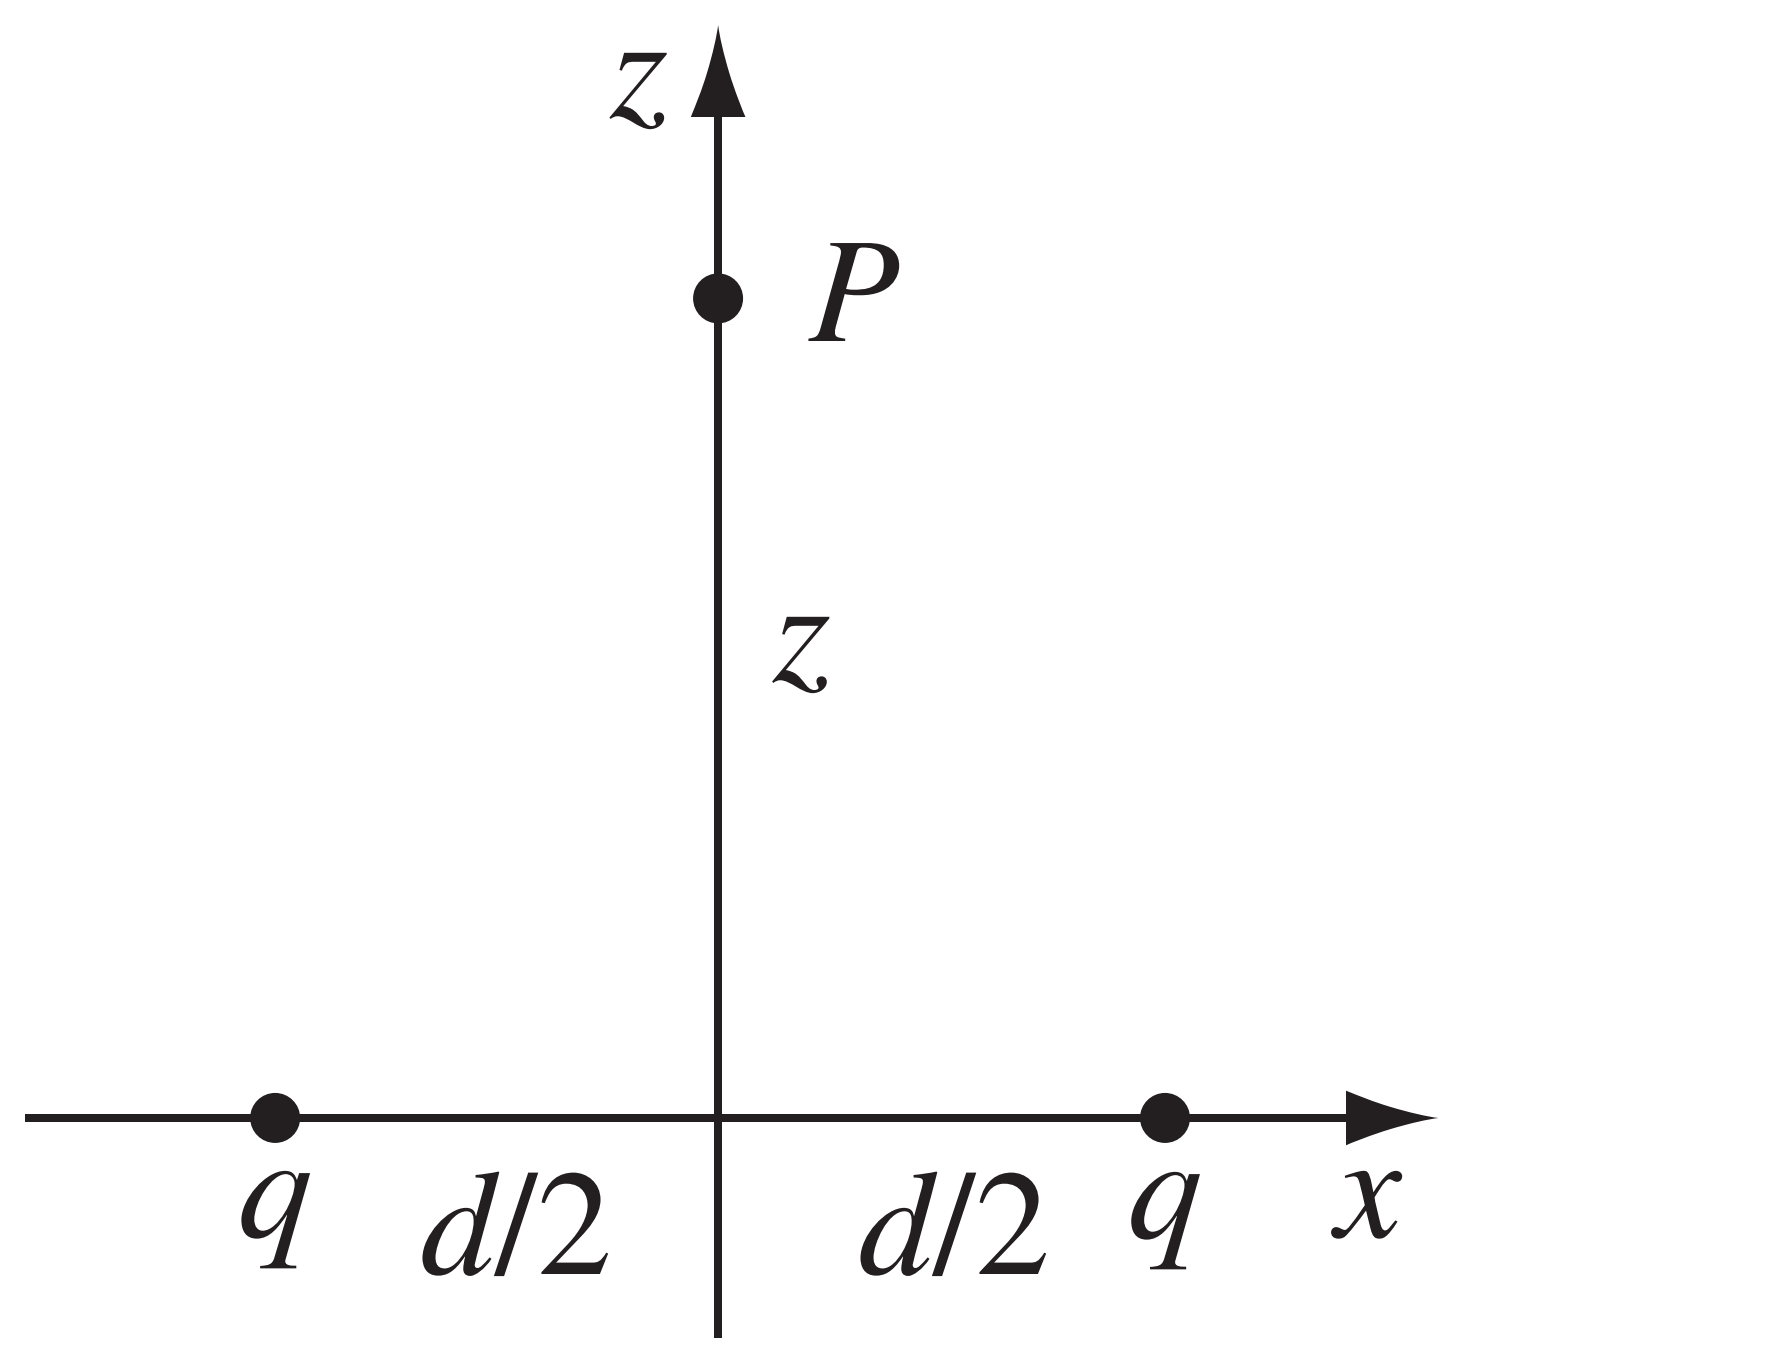
\includegraphics[width=0.4\textwidth]{../Rss/Electromagnetism/Electrostatics/Charge1.png}
        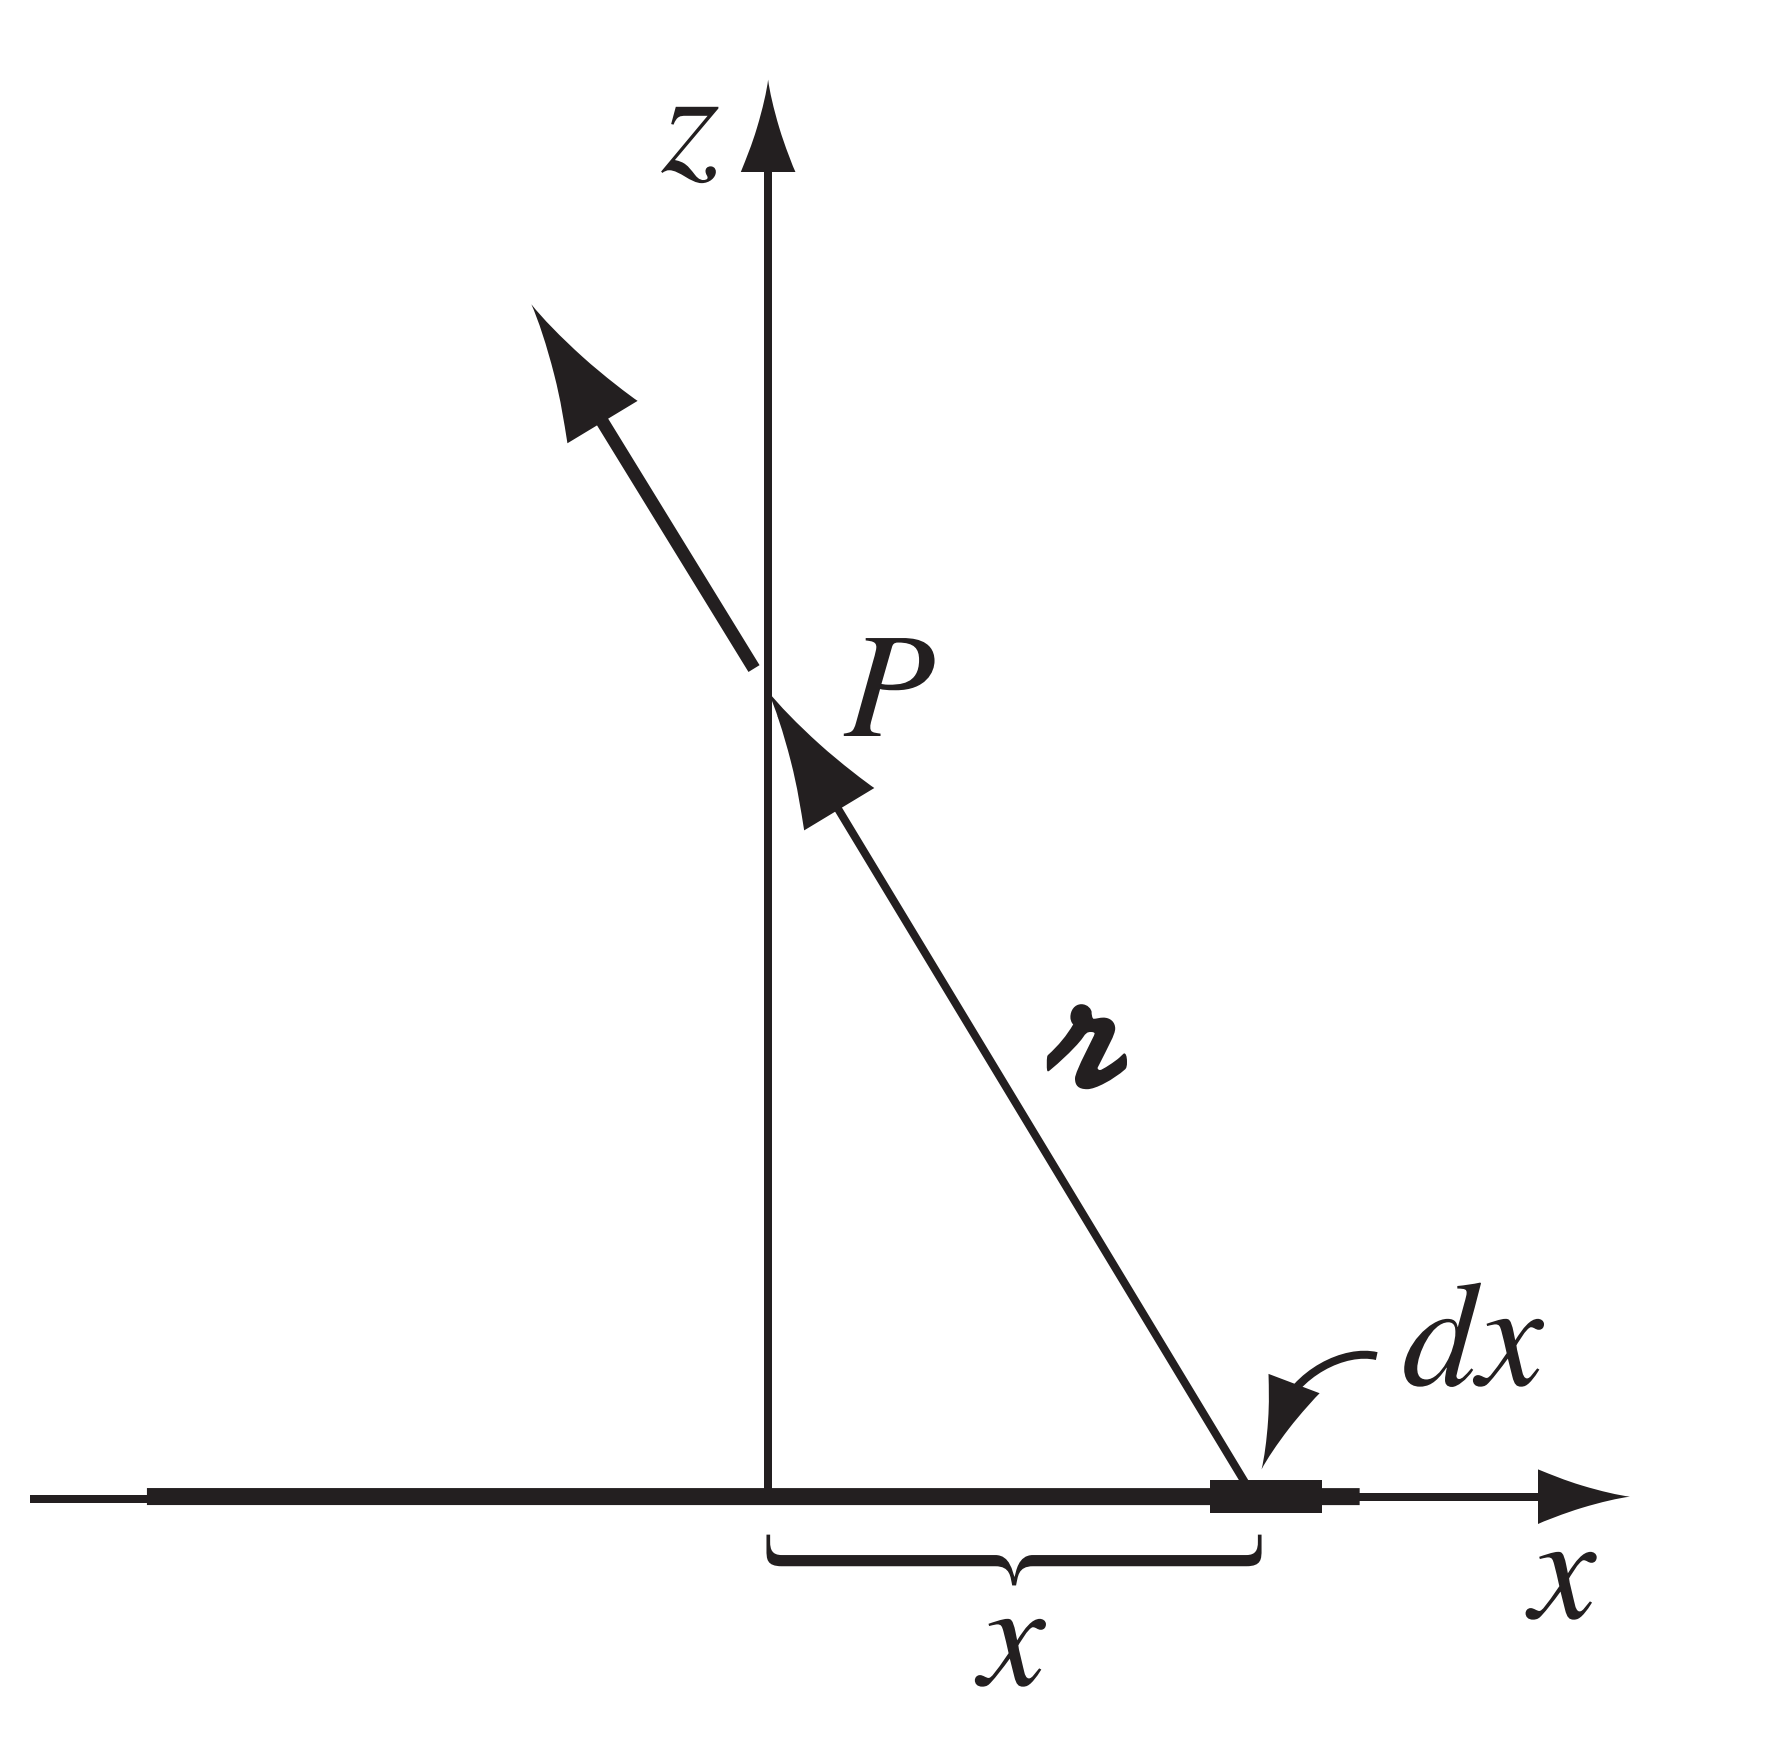
\includegraphics[width=0.4\textwidth]{../Rss/Electromagnetism/Electrostatics/Charge2.png}
        \caption*{Figure: Discreet charges and continuous line charge}
    \end{figure*}
First we need to determine the separation vector. Let's say the right one is $q_1$ while the left one is $q_2$. Thus, for $q_1$
\begin{align*}
    \brcurs_1&=\mathbf{r}- \mathbf{r'}=z\mathbf{\hat{z}}-(d/2)\mathbf{\hat{x}}\\
    \rcurs_1^2&=z^2+(d/2)^2\\
    \hrcurs&=\frac{\rcurs}{|\rcurs|}=\frac{\rcurs}{\sqrt{\rcurs^2}}=\frac{z\mathbf{\hat{z}}-(d/2) \mathbf{\hat{x}}}{\sqrt{z^2+(d/2)^2}}
\end{align*}
and for $q_2$
\begin{align*}
    \brcurs_1&=z\mathbf{\hat{z}}+(d/2)\mathbf{\hat{x}}\\
    \rcurs_1^2&=z^2+(d/2)^2\\
    \hrcurs&=\frac{z\mathbf{\hat{z}}+(d/2)\mathbf{\hat{x}}}{\sqrt{z^2+(d/2)^2}}
\end{align*}
Applying superposition theorem,
\begin{align*}
    \mathbf{E}&=\frac{1}{4\pi \epsilon_0}\sum_{i=1}^{2}\frac{q_i}{\rcurs_i^2}\hrcurs\\
    &=\frac{1}{4\pi \epsilon_0}\Biggl( \frac{q}{z^2+(d/2)^2}\frac{z\mathbf{\hat{z}}-(d/2)\mathbf{\hat{x}}}{\sqrt{z^2+(d/2)^2}} - \frac{q}{z^2+(d/2)^2} \frac{z\mathbf{\hat{z}}+(d/2)\mathbf{\hat{x}}}{\sqrt{z^2+(d/2)^2}}\Biggr)\\
    &=\frac{1}{4\pi \epsilon_0}\frac{2qz}{(z^2+(d/2)^2)^{3/2}}\mathbf{\hat{z}}
\end{align*}

\subsubsection*{Continuous line charge.} Find the electric field a distance $z$ above the midpoint of a straight line segment of length $2L$ that carries a uniform line charge $\lambda$. As always, we will find the separation vector first
\begin{align*}
    \rcurs&=z\mathbf{\hat{z}}- x\mathbf{\hat{x}}\\
    |\rcurs|^2&=z^2+x^2\\
    \hrcurs&=\frac{z\mathbf{\hat{z}}- x\mathbf{\hat{x}}}{(z^2+x^2)^{1/2}}
\end{align*}
Thus, the electric field is
\begin{align*}
    \mathbf{E}&=\frac{1}{4\pi\epsilon_0}\int_{-L}^{L}\frac{\lambda}{(z^2+x^2)} \frac{z \mathbf{\hat{z}}- x\mathbf{\hat{x}}}{(z^2+x^2)^{1/2}} \; dx\\
    &=\frac{\lambda}{4\pi\epsilon_0} \int_{-L}^{L}\frac{z \mathbf{\hat{z}}- x\mathbf{\hat{x}}}{(z^2+x^2)^{3/2}} \; dx\\
    &=\frac{\lambda}{4\pi\epsilon_0} \biggl[ z \mathbf{\hat{z}} \int_{-L}^{L} \frac{dx}{(z^2+x^2)^{3/2}} -  \mathbf{\hat{x}} \int_{-L}^{L} \frac{x}{(z^2+x^2)^{3/2}}\;dx\biggr]
\end{align*}
The first integral 
\begin{equation*}
    I_1=z \mathbf{\hat{z}} \int_{-L}^{L} \frac{dx}{(z^2+x^2)^{3/2}} 
\end{equation*}
can be easily solved using trig substitution. Substituting
\begin{equation*}
    \tan \theta=\frac{x}{z}
\end{equation*}
solving for $x$ and $dx$
\begin{equation*}
    x=z\tan\theta\qquad dx=z\sec^2 \theta\;d\theta
\end{equation*}
Based on the substitution, we also get
\begin{align*}
    \sec\theta&=\frac{(z^2+x^2)^{1/2}}{z}\\
    (z^2+x^2)^{3/2}&=z^3\sec^3\theta
\end{align*}
and
\begin{equation*}
    \sin \theta=\frac{x}{(z^2+x^2)^{1/2}}
\end{equation*}
We finally get all the equation we need
\begin{align*}
    I_1&=z \mathbf{\hat{z}} \int_{-L}^{L} \frac{z\sec^2 \theta\;d\theta}{z^3\sec^3\theta} \\
    &=\frac{\mathbf{\hat{z}}}{z} \int_{-L}^{L}\cos \theta\;d\theta\\
    &=\frac{\mathbf{\hat{z}}}{z}\sin\theta\bigg|_{-L}^{L}\\
    &=\frac{\mathbf{\hat{z}}}{z} \frac{x}{(z^2+x^2)^{1/2}}\bigg|_{-L}^{L}\\
    I_1&=2 \frac{L}{z(z^2+L^2)^{1/2}}\mathbf{\hat{z}}
\end{align*}
For second integral, simple u-sub is enough
\begin{align*}
    u&=z^2+x^2\\
    du&= 2x\;dx
\end{align*}
then\begin{align*}
    I_2&=- \mathbf{\hat{x}} \int_{-L}^{L} \frac{x}{(z^2+x^2)^{3/2}}\;dx\\
    &=\int_{-L}^{L} u^{-3/2}\;du\\
    &=\mathbf{\hat{x}}\frac{1 }{(z^2+x^2)^{1/2}} \bigg|_{-L}^{L}\\
    I_2&=0
\end{align*}
Substituting back
\begin{equation*}
    \mathbf{E}=2 \frac{\lambda}{4\pi\epsilon_0}\frac{L}{z(z^2+L^2)^{1/2}}\mathbf{\hat{z}}
\end{equation*}
For $L\rightarrow\infty$ carries\begin{equation*}
    \mathbf{E}_{L\rightarrow\infty}=\frac{\lambda}{2\pi \epsilon_0}\mathbf{\hat{z}}
\end{equation*}

\subsection*{Appendix: PR Listrik Magnet 27 Agustus 2024}
\subsubsection*{Soal 1.} Vector pemisahan $\brcurs$ (Gambar 1) dari titik sumber $r'$ ke titik medan $P$ adalah
\begin{equation*}
    \brcurs=\mathbf{P}-\mathbf{r'}=z\boldsymbol{\hat{z}}-(x\boldsymbol{\hat{x}}+y\boldsymbol{\hat{y}})=z\boldsymbol{\hat{z}}-x\boldsymbol{\hat{x}}-y\boldsymbol{\hat{y}}
\end{equation*}
sehingga nilai kuadrat dan vektor satuan adalah
\begin{align*}
    \rcurs^2&=\brcurs\cdot\brcurs=x^2+y^2+z^2\\
    \hrcurs&=\frac{\brcurs}{\sqrt{\rcurs^2}}=\frac{z\boldsymbol{\hat{z}}-x\boldsymbol{\hat{x}}-y\boldsymbol{\hat{y}}}{(x^2+y^2+z^2)^{1/2}}
\end{align*}
Selanjutnya, nilai $\mathbf{E}$ akibat lempengan persegi adalah
\begin{align*}
    \mathbf{E}&=\frac{1}{4\pi\epsilon_0}\int_{\mathcal{A}}\frac{\sigma}{\rcurs^2}\hrcurs\;da\\
    &=\frac{\sigma}{4\pi\epsilon_0} \int_{\mathcal{A}} \frac{1}{(x^2+y^2+z^2)} \frac{z\boldsymbol{\hat{z}}-x\boldsymbol{\hat{x}}-y\boldsymbol{\hat{y}}}{(x^2+y^2+z^2)^{1/2}}\;da\\
    &=\frac{\sigma}{4\pi\epsilon_0} \int_{-a/2}^{a/2} \int_{-a/2}^{a/2} \frac{z\boldsymbol{\hat{z}}-x\boldsymbol{\hat{x}}-y\boldsymbol{\hat{y}}}{(x^2+y^2+z^2)^{3/2}}\;dxdy
\end{align*}
Karena medan listrik komponen $x$ dan $y$ saling membatalkan, maka suku $-x\boldsymbol{\hat{x}}-y\boldsymbol{\hat{y}}$ dapat dihilangkan. Sehingga, integral dapat disederhanakan menjadi
\begin{equation*}
    \mathbf{E}=\frac{\sigma}{4\pi\epsilon_0} \int_{-a/2}^{a/2} \int_{-a/2}^{a/2} \frac{z\boldsymbol{\hat{z}}}{(x^2+y^2+z^2)^{3/2}}\;dxdy
\end{equation*}
\begin{figure}[ht]
    \centering
    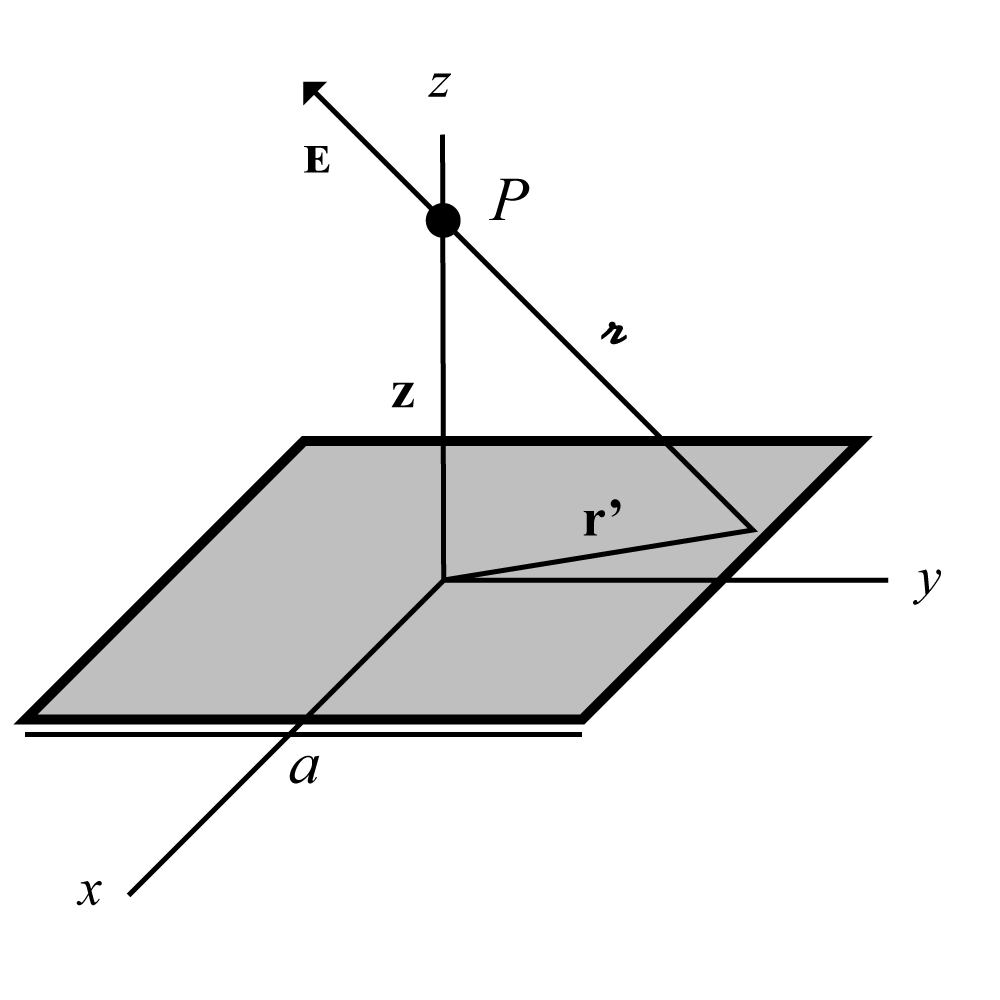
\includegraphics[width=0.4\textwidth]{../Rss/Electromagnetism/Electrostatics/Sqrt.png}
    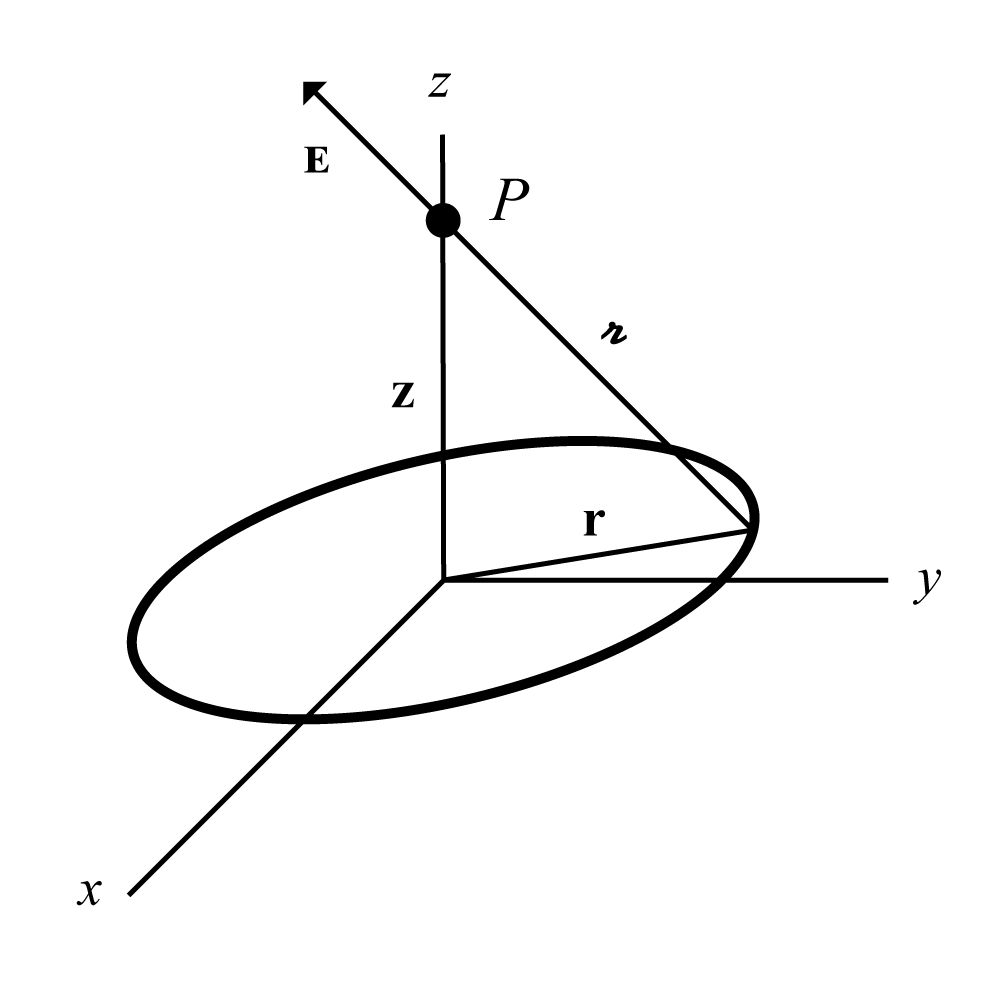
\includegraphics[width=0.4\textwidth]{../Rss/Electromagnetism/Electrostatics/Circ.png}
    \caption*{Gambar 1: Medan listrik akibat lempengan persegi (kiri) dan cincin lingkaran (kanan)}
\end{figure}
Melihat tabel integral, integral pertama adalah
\begin{align*}
    \mathbf{E}&=\frac{\sigma}{4\pi\epsilon_0} \int_{-a/2}^{a/2} \biggl(\frac{z\boldsymbol{\hat{z}}\;x}{(y^2+z^2)(x^2+y^2+z^2)^{1/2}}\Bigg|_{-a/2}^{a/2}\biggr)\;dy\\
    &=\frac{\sigma}{4\pi\epsilon_0} \int_{-a/2}^{a/2} \frac{z\boldsymbol{\hat{z}}\;a}{(y^2+z^2)(a^2/4+y^2+z^2)^{1/2}}\;dy
\end{align*}
Menggunkan komputer, integral dapat dievaluasi menjadi
\begin{align*}
    \mathbf{E}&=\frac{\sigma}{4\pi\epsilon_0} 2\boldsymbol{\hat{z}}\arctan\biggl(\frac{ay}{z(a^2+4y^2+z^2)^{1/2}}\biggr)\Bigg|_{-a/2}^{a/2}\\
    \mathbf{E}&=\frac{\sigma}{4\pi\epsilon_0} 2\boldsymbol{\hat{z}}\Bigg[ \arctan\biggl(\frac{a^2}{2z(a^2+a^2+z^2)^{1/2}}\biggr)\\& -\arctan\biggl(-\frac{a^2}{2z(a^2+a^2+z^2)^{1/2}}\biggr)\Bigg]
\end{align*}
Karena $\arctan $ merupakan fungsi ganjil, maka $\arctan -x=-\arctan x$. Dengan demikian
\begin{align*}
    \mathbf{E}&=\frac{\sigma}{4\pi\epsilon_0} 2\boldsymbol{\hat{z}}\cdot2\arctan\biggl(\frac{a^2}{2z(2a^2+z^2)^{1/2}}\biggr)\\
    &=\frac{\sigma}{\pi\epsilon_0} \arctan\biggl(\frac{a^2}{2z(2a^2+z^2)^{1/2}}\biggr) \boldsymbol{\hat{z}}
\end{align*}
Sebagai cek, limit ketika $a\rightarrow\infty$ adalah bidang menjadi tak hingga dengan besar medan listrik $\mathbf{E}=\sigma/(2\epsilon_0)$. Persamaan tersebut menunjukan
\begin{align*}
    \mathbf{E}_{a\rightarrow\infty}&=\lim_{a\rightarrow\infty}\frac{\sigma}{\pi\epsilon_0} \arctan\biggl(\frac{a^2}{2z(2a^2+z^2)^{1/2}}\biggr) \boldsymbol{\hat{z}}\\
    &=\frac{\sigma}{\pi\epsilon_0} \frac{\pi}{2}\\
    \mathbf{E}_{a\rightarrow\infty}&=\frac{\sigma}{2\epsilon_0} 
\end{align*}
Sesuai dengan medan listik oleh bidang tak hingga.

\subsubsection*{Soal 2.} Vector pemisahan $\brcurs$ (Gambar 1) dari titik sumber $r$ ke titik medan $P$ adalah
\begin{equation*}
    \brcurs=\mathbf{P}-\mathbf{r}= z\boldsymbol{\hat{z}}- (r\boldsymbol{\hat{r}}+\theta\boldsymbol{\hat{\theta}})= z\boldsymbol{\hat{z}}- r\boldsymbol{\hat{r}} -\theta\boldsymbol{\hat{\theta}}
\end{equation*}
dalam koordinat tabung. Sehingga nilai kuadrat dan vektor satuan adalah
\begin{align*}
    |\rcurs^2|&=\brcurs\cdot\brcurs=r^2+z^2\\
    \hrcurs&=\frac{\brcurs}{\sqrt{\rcurs^2}}=\frac{z\boldsymbol{\hat{z}}- r\boldsymbol{\hat{r}} -\theta\boldsymbol{\hat{\theta}}}{(r^2+z^2)^{1/2}}
\end{align*}
Perpindahan $dl$ dalam koordinat tabung adalah $dl=r\;dr+r\theta\;d\theta+z\;dz$. Karena integrasi akan dilakukan sepanjang keliling lingkaran, $r$ dan $z$ adalah konstan. Sehingga, $dl= r\theta\;d\theta$. Maka medan listrik akibat cincin lingkaran adalah:
\begin{align*}
    \mathbf{E}&=\frac{1}{4\pi\epsilon_0} \int_{l}\frac{\lambda}{\rcurs^2}\hrcurs\;dl\\
    &=\frac{1}{4\pi\epsilon_0} \oint \frac{1}{(r^2+z^2)} \frac{z\boldsymbol{\hat{z}}- r\boldsymbol{\hat{r}} -\theta\boldsymbol{\hat{\theta}}}{(r^2+z^2)^{1/2}} \lambda r\;d\theta\\
    \mathbf{E}&=\frac{1}{4\pi\epsilon_0} \oint \frac{\lambda r (z\boldsymbol{\hat{z}}- r\boldsymbol{\hat{r}} -\theta\boldsymbol{\hat{\theta}})}{(r^2+z^2)^{3/2}}\;d\theta
\end{align*}
Karena medan listrik komponen $r$ dan $\theta$ saling membatalkan, maka suku $- r\boldsymbol{\hat{r}} -\theta\boldsymbol{\hat{\theta}}$ dapat dihilangkan. Sehingga, integral dapat disederhanakan menjadi
\begin{equation*}
    \mathbf{E}=\frac{1}{4\pi\epsilon_0} \oint \frac{\lambda r \;z\boldsymbol{\hat{z}}}{(r^2+z^2)^{3/2}}\;d\theta
\end{equation*}
Melihat tabel integral, integral adalah
\begin{align*}
    \mathbf{E}&=\frac{1}{4\pi\epsilon_0}\lambda r \;z\boldsymbol{\hat{z}} \frac{\theta}{(r^2+z^2)^{3/2}}\bigg|_{0}^{2\pi}\\
    \mathbf{E}&=\frac{z\boldsymbol{\hat{z}}}{4\pi\epsilon_0}  \frac{\lambda2\pi r}{(r^2+z^2)^{3/2}}
\end{align*}
Mengingat bahwa $\lambda2\pi r=Q$, dimana $Q$ adalah muatan total; maka
\begin{equation*}
    \mathbf{E}=\frac{1}{4\pi\epsilon_0}  \frac{Qz}{(r^2+z^2)^{3/2}}\boldsymbol{\hat{z}}
\end{equation*}
\end{document}